% Files should be in encoding corresponding to the setting of \usepackage[...]{inputenc}

\documentclass[%      Basic settings of the document
%  draft,    				  % Turn on draft compilation
  12pt,       				% 12 points default font size
  a4paper,    				% Paper format A4
  %oneside,      			% One-sided print
	twoside,      			% Two-sided print (chapters and other important blocks begin at odd-numbered pages)
	unicode,						% Bookmarks and metainformation in the compiled PDF will be unicode
]{report}				    	% Report class, suitable for typesetting theses

\usepackage[utf8]		  %	The input files are in UTF-8 (unicode)
	{inputenc}					% Package for setting input encoding

\usepackage[				    % Geometry of the pages
	bindingoffset=10mm,		% Binding offset
	hmargin={25mm,25mm},	% Inner and outer margins
	vmargin={25mm,34mm},	% Upper and lower margins
	footskip=17mm,			  % Footskip size
	nohead,					      % No header
	marginparsep=2mm,		  % Margin separation amount
	marginparwidth=18mm,	% Width of the text margins
]{geometry}

\usepackage{sectsty}
	%sets all (sub)section headers to sans-serif type,
	%except for \chapter, for which the setting is done separately in thesis.sty
	\allsectionsfont{\sffamily}

\usepackage{graphicx} % Package for inclusion of external graphics
						

\usepackage[
	nohyperlinks				% No hyperlinks to the list of acronyms will be created
]{acronym}						% Package 'acronym' for automated handling of abbreviations and symbols
											% Neccessary for the 'acronym' environment of 'thesis' to work

\usepackage[
	breaklinks=true,		% Hypertext links can be line-broken
	hypertexnames=false % Names of hypertextlinks will be
											% independent of TeX labels
]{hyperref}						% Package 'hyperref' for the support of hypertext link
											% Neccessary for the 'pdfsettings' command of 'thesis' package

\usepackage{pdfpages} % Package allowing including pages from external PDFs
                      % Neccessary for appending the PDF of the title page etc.,
											% which are generated by the BUT information system

\usepackage{enumitem} % Package for handling spacing in itemization environments
  \setlist{topsep=0pt,partopsep=0pt,noitemsep}

\usepackage{cmap} 		% This package allows the final PDF
											% is fully "searchable" and "copyable"

%\usepackage{upgreek}	% Package for typesetting roman-type greek letters
											%% e.g. upright pi: \uppi
											%% e.g. upright mu: \upmu (usable in micrometers, for instance)
											%% be aware of the graphical incompatibility with the default Computer Modern fonts!

\usepackage{dirtree}	% Printing the directory tree
                      % useful for detailing the stuff that is included on the additional medium like CD

\usepackage[formats]{listings}	% Package enabling inclusion of computer codes
\lstset{
%	Definition of the programming language
% language=[LaTeX]{TeX},	% LaTeX
%	language={Matlab},		  % Matlab
	language={C},           % C
    basicstyle=\ttfamily,	% basic font type
    tabsize=2,			      % with of the tab
    inputencoding=utf8,   % character encoding of the files that will be included
		columns=fixed,        % choose fixed or flexible,
		fontadjust=true       % adjusting the columns
    extendedchars=true,
    literate=%              definition of symbols with diacritics
    {á}{{\'a}}1
    {č}{{\v{c}}}1
    {ď}{{\v{d}}}1
    {é}{{\'e}}1
    {ě}{{\v{e}}}1
    {í}{{\'i}}1
    {ň}{{\v{n}}}1
    {ó}{{\'o}}1
    {ř}{{\v{r}}}1
    {š}{{\v{s}}}1
    {ť}{{\v{t}}}1
    {ú}{{\'u}}1
    {ů}{{\r{u}}}1
    {ý}{{\'y}}1
    {ž}{{\v{z}}}1
    {Á}{{\'A}}1
    {Č}{{\v{C}}}1
    {Ď}{{\v{D}}}1
    {É}{{\'E}}1
    {Ě}{{\v{E}}}1
    {Í}{{\'I}}1
    {Ň}{{\v{N}}}1
    {Ó}{{\'O}}1
    {Ř}{{\v{R}}}1
    {Š}{{\v{S}}}1
    {Ť}{{\v{T}}}1
    {Ú}{{\'U}}1
    {Ů}{{\r{U}}}1
    {Ý}{{\'Y}}1
    {Ž}{{\v{Z}}}1
}

%%%%%%%%%%%%%%%%%%%%%%%%%%%%%%%%%%%%%%%%%%%%%%%%%%%%%%%%%%%%%%%%%
%%%%%%%%                   Definitions                 %%%%%%%%%%
%%%%%%%%%%%%%%%%%%%%%%%%%%%%%%%%%%%%%%%%%%%%%%%%%%%%%%%%%%%%%%%%%

% Variable fields such as your name, title of the thesis atc. are set in this file.
% The file is SHARED between the thesis text and the presentation --- no need to set anything twice.

\usepackage[
  english,			% English study program
%%% Choose one of the thesis types
	semestral,		%	semestral project (abstracts, declaration and acknowledgements are excluded) (default)
  %bachelor,			%	Bachelor's thesis
  %master,			% Master's thesis
  %treatise,			% Treatise on doctoral thesis
  %doctoral,				% Doctoral thesis
%%% Choose one of the options:
%  left,				% Equations and captions will be aligned to the left
  center,			% Equations and captions will be centered (default)
]{thesis}   % Package for typesetting theses


%%% First and last name of the thesis author, following the scheme
% [titles in front]{FirstName}{LastName}[titles after]
% If the author does not have a title in front/after, just delete the entire string '[...]'
\author[Bc.]{FirstName}{LastName}

%%% Brno University of Technology identification number of author (BUT ID)
\butid{007}

%%% First and last name of the advisor
% [titles in front]{FirstName}{LastName}[titles after]
% If the author does not have a title in front/after, just delete the entire string '[...]'
% [titles in front]{FirstName}{LastName}[titles after]
\advisor[prof.\ Ing.]{FirstName}{LastName}[CSc.]

%%% First and last name of the opponent
% [titles in front]{FirstName}{LastName}[titles after]
% Makes use only in the presentation for defense;
% in case you do not want the opponent to be shown on the title slide, just comment out the command
% The opponent is not shown in case of the semestral thesis (no opponent exists actually at that time)
% In the case of a doctoral thesis, two to three oponents are typically involved. In such a case, if you want to have them on the title slide, please go to the definition of "VUT title page" in the thesis.sty file, uncomment and adapt their names.
\opponent[doc.\ Mgr.]{FirstName}{LastName}[Ph.D.]

%%% Thesis title
%  In the case of a very long thesis title, it may happen that it does not fit
%  into the slot in the footbar of the slides. You may use the command
%  \def\insertshorttitle{Shortened th.\ title}
%  where the shortened version of the title appears as the parameter.
%  If you do not want to shorten the title, you will have to redefine how the slide footbar
%  is generated, see: https://bit.ly/3EJTp5A
\title{Title of Student's Thesis}

%%% Study program/specialization
\specialization{Teleinformatics} %Teleinformatika

%%% Department
%\department{Department of Control and Instrumentation}  %Ústav automatizace a měřicí techniky
%\department{Department of Biomedical Engineering}       %Ústav biomedicínského inženýrství
%\department{Department of Electrical Power Engineering} %Ústav elektroenergetiky
%\department{Department of Electrical and Electronic Technology}   %Ústav elektrotechnologie
%\department{Department of Physics}                      %Ústav fyziky
%\department{Department of Foreign Languages}            %Ústav jazyků
%\department{Department of Mathematics}                  %Ústav matematiky
%\department{Department of Microelectronics}             %Ústav mikroelektroniky
%\department{Department of Radio Electronics}            %Ústav radioelektroniky
%\department{Department of Theoretical and Experimental Electrical Engineering}  %Ústav teoretické a experimentální elektrotechniky
\department{Department of Telecommunications}           %Ústav telekomunikací
%\department{Department of Power Electrical and Electronic Engineering}   %Ústav výkonové elektrotechniky a elektroniky

%%% Faculty
%\faculty{Faculty of Architecture}   %Fakulta architektury
\faculty{Faculty of Electrical Engineering and~Communication}   %Fakulta elektrotechniky a~komunikačních technologií
%\faculty{Faculty of Chemistry}   %Fakulta chemická
%\faculty{Faculty of Information Technology}   %Fakulta informačních technologií
%\faculty{Faculty of Business and Management}   $Fakulta podnikatelská
%\faculty{Faculty of Civil Engineering}   %Fakulta stavební
%\faculty{Faculty of Mechanical Engineering}   %Fakulta strojního inženýrství
%\faculty{Faculty of Fine Arts}   %Fakulta výtvarných umění
%
%Logotype selection (in square brackets short logo, in curly brackets full logo):
\facultylogo[logo/FEEC_abbreviation_color_PANTONE_EN]{logo/UTKO_color_PANTONE_EN}


%%% Graduate year (typically the calendar year of the defense)
\graduateyear{2033}
%%% Academic year (typically the year of solution of the thesis in the format n/n+1)
\academicyear{2032/33}
% Date of the defense (makes use only in the presentation slides)
\date{15 June 2033} 

%%% Place of the defense
\city{Brno}

%%% Abstract
\abstract{%
Abstract in English.
}

%%% Keywords
\keywrds{%
Keywords in English
}

%%% Thanks and acknowledgement
\acknowledgement{%
I would like to thank the advisor of my thesis, Ing.~XXX YYY, Ph.D.\ for his/her valuable comments etc.
}%  % please go into that file and fill information about you, your topic etc.



%%%%%%%%%%%%%%%%%%%%%%%%%%%%%%%%%%%%%%%%%%%%%%%%%%%%%%%%%%%%%%%%%%%%%%%%
%%%%%   Setting values that appear in the Properties of the PDF  %%%%%%%
%%%%%%%%%%%%%%%%%%%%%%%%%%%%%%%%%%%%%%%%%%%%%%%%%%%%%%%%%%%%%%%%%%%%%%%%
%% If 'hyperref' package is loaded then command '\pdfsettings' can be simply used
\pdfsettings
%  However, you can set the individual fields by hand:
%\hypersetup{
%  pdftitle={Title of the thesis},    	% 'Document Title' field
%  pdfauthor={Author name},   	        % 'Author' field
%  pdfsubject={Type of the document},  	% 'Subject' field
%  pdfkeywords={Keywords}           	  % 'Keywords' field
%}
%%%%%%%%%%%%%%%%%%%%%%%%%%%%%%%%%%%%%%%%%%%%%%%%%%%%%%%%%%%%%%%%%%%%%%%

\pdfmapfile{=vafle.map}

%%%%%%%%%%%%%%%%%%%%%%%%%%%%%%%%%%%%%%%%%%%%%%%%%%%%%%%%%%%%%%%%%%%%%%%
%%%%%%%%%%%     Actual start of the document      %%%%%%%%%%%%%%%%%%%%%
%%%%%%%%%%%%%%%%%%%%%%%%%%%%%%%%%%%%%%%%%%%%%%%%%%%%%%%%%%%%%%%%%%%%%%%
\begin{document}
\pagestyle{empty}      %avoiding page numbering for the moment

%%%% Include the cover  --- Sept. 2021: the faculty wants to disable generating the cover
%\includepdf[pages=1]%  either by using PDF generated by the information system
  %{pdf/cover-example}% no spaces allowed in the filename!
%%%% OR the cover can be generated using
%%\makecover
%%%%
%\oddpage%  this command adds an empty page when two-side printing is selected
%% but in any case:
%\setcounter{page}{1} %reset the pagecounter --- the cover should not affect numbering

%%% Include the titlepage
\includepdf[pages=1]%    either by using PDF generated by the information system
  {pdf/titlepage-example}% no spaces allowed in the filename!
%%% OR the titlepage can be generated using
%\maketitle
%%%
\oddpage%    this command adds an empty page when two-side printing is selected
   
%%% Include the thesis assignment (goals)
\includepdf[pages=1]%   either by using PDF generated by the information system
  {pdf/assignment-example}% no spaces allowed in the filename!
%%% OR the empty page reserving the space for assignment can be generated using
%\patternpage{}%
%	{\sffamily\Huge\centering IN PLACE OF HERE\\ INSERT THE SHEET WITH THE THESIS ASSIGNMENT}%
%	{\sffamily\centering This page is here in order to keep page numbering correct}
%%%
\oddpage%   this command adds an empty page when two-side printing is selected

%%% Generate abstract
\makeabstract

%%% Generate declaration
\makedeclaration

%%% Generate page with thanks and acknowledgements
\makeacknowledgement

%%% Generate table of contents
\tableofcontents

%%% Generate list of figures
% (exclude such a list if it contains two or less items)
\listoffigures

%%% Generate list of tables
% (exclude such a list if it contains two or less items)
\listoftables

%%% Generate list of listings
% (exclude such a list if it contains two or less items)
\lstlistoflistings

\cleardoublepage\pagestyle{plain}   % turn page-numbering on

%Including chapters and appendices should be preferrably done with \include instead of \input
%%% Include the file with Introduction
\chapter*{Introduction}
\phantomsection
\addcontentsline{toc}{chapter}{Introduction}


%%% Include the file with Introduction
\chapter*{Aim of the thesis}
\phantomsection
\addcontentsline{toc}{chapter}{Aim of the thesis}

Specification of the objectives to be solved in the thesis.
If your study program does not insist on having such a~separate chapter with the aims,
please specify them as a~part of the Introduction.

%%% Include the file with the project solution
\chapter{Theory}

Theoretical background of the thesis comes now, suitably split into chapters and sections.

(The structure suggested in this template is the coarsest one.
Please discuss your particular structure with your adviser.)


%%% Include the file with the results
\chapter{Thesis Results}

Practical part and results of the student, suitably split into chapters and sections.

\section{Selection of Programming Language}
Lorem ipsum dolor sit amet, consectetuer adipiscing elit. Nulla pulvinar eleifend sem. Integer in sapien. Etiam sapien elit, consequat eget, tristique non, venenatis quis, ante. In laoreet, magna id viverra tincidunt, sem odio bibendum justo, vel imperdiet sapien wisi sed libero. Phasellus enim erat, vestibulum vel, aliquam a, posuere eu, velit. Aliquam erat volutpat. Nullam faucibus mi quis velit \cite{sr02/2009}.

\section{Implementation}
Fusce tellus odio, dapibus id fermentum quis, suscipit id erat. Fusce tellus. Morbi scelerisque luctus velit. In laoreet, magna id viverra tincidunt, sem odio bibendum justo, vel imperdiet sapien wisi sed libero. Quisque porta. Fusce suscipit libero eget elit. Nulla non lectus sed nisl molestie malesuada. Phasellus faucibus molestie nisl. Integer vulputate sem a nibh rutrum consequat. Proin mattis lacinia justo. Phasellus et lorem id felis nonummy placerat. Etiam ligula pede, sagittis quis, interdum ultricies, scelerisque eu. Cras elementum. Aenean placerat. Donec ipsum massa, ullamcorper in, auctor et, scelerisque sed, est. Aliquam ante. Integer imperdiet lectus quis justo. Vivamus ac leo pretium faucibus. Nullam faucibus mi quis velit.

\subsection{Tests and Evaluation}
Neque porro quisquam est, qui dolorem ipsum quia dolor sit amet, consectetur, adipisci velit, sed quia non numquam eius modi tempora incidunt ut labore et dolore magnam aliquam quaerat voluptatem. Aliquam erat volutpat. Lorem ipsum dolor sit amet, consectetuer adipiscing elit \cite{sr02/2009,pravidla}. Nunc auctor. Neque porro quisquam est, qui dolorem ipsum quia dolor sit amet, consectetur, adipisci velit, sed quia non numquam eius modi tempora incidunt ut labore et dolore magnam aliquam quaerat voluptatem. Maecenas lorem. Maecenas libero. In laoreet, magna id viverra tincidunt, sem odio bibendum justo, vel imperdiet sapien wisi sed libero. Nullam rhoncus aliquam metus.

\subsubsection{Integer rutrum orci vestibulum}
Integer rutrum, orci vestibulum ullamcorper ultricies, lacus quam ultricies odio, vitae placerat pede sem sit amet enim. Ut enim ad minim veniam, quis nostrud exercitation ullamco laboris nisi ut aliquip ex ea commodo consequat. Fusce tellus odio, dapibus id fermentum quis, suscipit id erat. Nullam eget nisl. Nunc auctor. Etiam dui sem, fermentum vitae, sagittis id, malesuada in, quam. Fusce dui leo, imperdiet in, aliquam sit amet, feugiat eu, orci. Curabitur vitae diam non enim vestibulum interdum. Aliquam erat volutpat. Pellentesque sapien. Phasellus enim erat, vestibulum vel, aliquam a, posuere eu, velit.

\subsubsection{Eger rutrum orci westibulum}
Fusce dui leo, imperdiet in, aliquam sit amet, feugiat eu, orci. Maecenas aliquet accumsan leo. Aliquam ornare wisi eu metus. Cum sociis natoque penatibus et magnis dis parturient montes, nascetur ridiculus mus. Aliquam erat volutpat. Donec iaculis gravida nulla. Sed elit dui, pellentesque a, faucibus vel, interdum nec, diam. Temporibus autem quibusdam et aut officiis debitis aut rerum necessitatibus saepe eveniet ut et voluptates repudiandae sint et molestiae non recusandae. Nulla non arcu lacinia neque faucibus fringilla. Phasellus enim erat, vestibulum vel, aliquam a, posuere eu, velit. Praesent vitae arcu tempor neque lacinia pretium
\cite{Walter1999,Svacina1999IEEE,RajmicSysel2002}.

Aliquam erat volutpat. Quisque porta. Integer imperdiet lectus quis justo. Nullam justo enim, consectetuer nec, ullamcorper ac, vestibulum in, elit. Nullam faucibus mi quis velit. Fusce tellus. Fusce consectetuer risus a nunc. Cras pede libero, dapibus nec, pretium sit amet, tempor quis. Morbi imperdiet, mauris ac auctor dictum, nisl ligula egestas nulla, et sollicitudin sem purus in lacus
\cite{CSN_ISO_690-2011,CSN_ISO_7144-1997,CSN_ISO_31-11}.
Mauris elementum mauris vitae tortor. Neque porro quisquam est, qui dolorem ipsum quia dolor sit amet, consectetur, adipisci velit, sed quia non numquam eius modi tempora incidunt ut labore et dolore magnam aliquam quaerat voluptatem. Quisque porta. Integer vulputate sem a nibh rutrum consequat. Nulla pulvinar eleifend sem. Praesent id justo in neque elementum ultrices \cite{BiernatovaSkupa2011:CSNISO690komentar}.

Fusce suscipit libero eget elit. Integer vulputate sem a nibh rutrum consequat. Aliquam erat volutpat. Etiam neque. Nulla turpis magna, cursus sit amet, suscipit a, interdum id, felis. Nullam rhoncus aliquam metus. Etiam dui sem, fermentum vitae, sagittis id, malesuada in, quam. Nunc auctor. Nunc dapibus tortor vel mi dapibus sollicitudin. Praesent in mauris eu tortor porttitor accumsan. Nulla non arcu lacinia neque faucibus fringilla. Nullam lectus justo, vulputate eget mollis sed, tempor sed magna. Maecenas lorem. Aenean placerat. Donec vitae arcu. Maecenas lorem. Donec iaculis gravida nulla. Nulla non lectus sed nisl molestie malesuada.

Duis pulvinar. Nulla est. Duis condimentum augue id magna semper rutrum. Integer pellentesque quam vel velit. Aliquam ante. Nulla quis diam. Proin mattis lacinia justo. Aenean fermentum risus id tortor. Nunc auctor. Nullam justo enim, consectetuer nec, ullamcorper ac, vestibulum in, elit. In dapibus augue non sapien. Etiam bibendum elit eget erat. In sem justo, commodo ut, suscipit at, pharetra vitae, orci. Maecenas libero.

Nulla non lectus sed nisl molestie malesuada. Donec vitae arcu. Aenean fermentum risus id tortor. Praesent in mauris eu tortor porttitor accumsan. Nulla pulvinar eleifend sem. Duis viverra diam non justo. Integer imperdiet lectus quis justo. Pellentesque habitant morbi tristique senectus et netus et malesuada fames ac turpis egestas. In rutrum. Excepteur sint occaecat cupidatat non proident, sunt in culpa qui officia deserunt mollit anim id est laborum. Nulla non lectus sed nisl molestie malesuada. Aliquam erat volutpat. Mauris tincidunt sem sed arcu. Duis bibendum, lectus ut viverra rhoncus, dolor nunc faucibus libero, eget facilisis enim ipsum id lacus. Fusce tellus odio, dapibus id fermentum quis, suscipit id erat. In enim a arcu imperdiet malesuada. Nulla non lectus sed nisl molestie malesuada. Proin mattis lacinia justo.

Aliquam in lorem sit amet leo accumsan lacinia. Cum sociis natoque penatibus et magnis dis parturient montes, nascetur ridiculus mus. Duis sapien nunc, commodo et, interdum suscipit, sollicitudin et, dolor. Suspendisse sagittis ultrices augue. Nullam lectus justo, vulputate eget mollis sed, tempor sed magna. In convallis. Praesent id justo in neque elementum ultrices. Neque porro quisquam est, qui dolorem ipsum quia dolor sit amet, consectetur, adipisci velit, sed quia non numquam eius modi tempora incidunt ut labore et dolore magnam aliquam quaerat voluptatem.

Pellentesque pretium lectus id turpis. Nemo enim ipsam voluptatem quia voluptas sit aspernatur aut odit aut fugit, sed quia consequuntur magni dolores eos qui ratione voluptatem sequi nesciunt. Curabitur ligula sapien, pulvinar a vestibulum quis, facilisis vel sapien. Praesent dapibus. Sed elit dui, pellentesque a, faucibus vel, interdum nec, diam. Duis viverra diam non justo. Duis ante orci, molestie vitae vehicula venenatis, tincidunt ac pede. Phasellus rhoncus. Maecenas fermentum, sem in pharetra pellentesque, velit turpis volutpat ante, in pharetra metus odio a lectus. Proin pede metus, vulputate nec, fermentum fringilla, vehicula vitae, justo. Fusce aliquam vestibulum ipsum. Nullam at arcu a est sollicitudin euismod.

%Aliquam ante. Phasellus faucibus molestie nisl. Etiam ligula pede, sagittis quis, interdum ultricies, scelerisque eu. Morbi leo mi, nonummy eget tristique non, rhoncus non leo. Cum sociis natoque penatibus et magnis dis parturient montes, nascetur ridiculus mus. Morbi scelerisque luctus velit. Curabitur bibendum justo non orci. Donec quis nibh at felis congue commodo. Nullam faucibus mi quis velit. Aenean id metus id velit ullamcorper pulvinar. Pellentesque sapien. Fusce nibh. Vestibulum fermentum tortor id mi. Nullam eget nisl. Praesent vitae arcu tempor neque lacinia pretium. Proin in tellus sit amet nibh dignissim sagittis. Donec quis nibh at felis congue commodo.
%
%Nam quis nulla. Proin in tellus sit amet nibh dignissim sagittis. Nullam dapibus fermentum ipsum. Curabitur ligula sapien, pulvinar a vestibulum quis, facilisis vel sapien. Nam libero tempore, cum soluta nobis est eligendi optio cumque nihil impedit quo minus id quod maxime placeat facere possimus, omnis voluptas assumenda est, omnis dolor repellendus. Vivamus ac leo pretium faucibus. Nunc tincidunt ante vitae massa. Maecenas sollicitudin. Ut tempus purus at lorem. Nullam lectus justo, vulputate eget mollis sed, tempor sed magna. Fusce consectetuer risus a nunc. Etiam quis quam.
%
%Donec quis nibh at felis congue commodo. Sed vel lectus. Donec odio tempus molestie, porttitor ut, iaculis quis, sem. Nullam feugiat, turpis at pulvinar vulputate, erat libero tristique tellus, nec bibendum odio risus sit amet ante. Sed elit dui, pellentesque a, faucibus vel, interdum nec, diam. Cras elementum. Sed vel lectus. Donec odio tempus molestie, porttitor ut, iaculis quis, sem. Etiam neque. Integer tempor. Vivamus porttitor turpis ac leo. Nulla non arcu lacinia neque faucibus fringilla.
%
%Etiam posuere lacus quis dolor. Nemo enim ipsam voluptatem quia voluptas sit aspernatur aut odit aut fugit, sed quia consequuntur magni dolores eos qui ratione voluptatem sequi nesciunt. Nullam faucibus mi quis velit. Cum sociis natoque penatibus et magnis dis parturient montes, nascetur ridiculus mus. Phasellus faucibus molestie nisl. Maecenas ipsum velit, consectetuer eu lobortis ut, dictum at dui. Maecenas aliquet accumsan leo. Pellentesque ipsum. Donec vitae arcu. Suspendisse nisl. Morbi imperdiet, mauris ac auctor dictum, nisl ligula egestas nulla, et sollicitudin sem purus in lacus. Pellentesque ipsum. Ut enim ad minima veniam, quis nostrum exercitationem ullam corporis suscipit laboriosam, nisi ut aliquid ex ea commodi consequatur? Nam libero tempore, cum soluta nobis est eligendi optio cumque nihil impedit quo minus id quod maxime placeat facere possimus, omnis voluptas assumenda est, omnis dolor repellendus.


%%% Include the file with Conclusion
\chapter*{Conclusion}
\phantomsection
\addcontentsline{toc}{chapter}{Conclusion}

Thesis conclusion.


%%% Include the file with references
% For the list of references, use one of the two options below

%%%%%%%%%%%%%%%%%%%%%%%%%%%%%%%%%%%%%%%%%%%%%%%%%%%%%%%%%%%%%%%%%%%%%%%%%
%1) References created directly, by hand, using the 'thebibliography' environment

\begin{thebibliography}{99}
	
\bibitem{sr02/2009}
		VUT v~Brně:
    \emph{Úprava, odevzdávání a zveřejňování vysokoškolských kva\-li\-fi\-kač\-ních prací na VUT v~Brně}\/ [online].
		Směrnice rektora č.\,2/2009.
		Brno: 2009, po\-sled\-ní aktualizace 24.\,3.\,2009 [cit.\,23.\,10.\,2015].
    Dostupné z~URL:\\
    <\url{https://www.vutbr.cz/uredni-deska/vnitrni-predpisy-a-dokumenty/smernice-rektora-f34920/}>.

\bibitem{CSN_ISO_690-2011}
    \emph{ČSN ISO 690 (01 0197) Informace a dokumentace -- Pravidla pro bibliografické odkazy a citace informačních zdrojů.}
    40 stran. Praha: Český normalizační institut, 2011.

\bibitem{CSN_ISO_7144-1997}
    \emph{ČSN ISO 7144 (010161) Dokumentace -- Formální úprava disertací a podobných dokumentů.}
    24 stran. Praha: Český normalizační institut, 1997.

\bibitem{CSN_ISO_31-11}
    \emph{ČSN ISO 31-11 Veličiny a jednotky -- část 11: Matematické znaky a značky používané ve fyzikálních vědách a v~technice.}
    Praha: Český normalizační institut, 1999.

\bibitem{BiernatovaSkupa2011:CSNISO690komentar}
    BIERNÁTOVÁ, O., SKŮPA, J.:
    \emph{Bibliografické odkazy a citace dokumentů dle ČSN ISO 690 (01 0197) platné od 1.\,dubna 2011}\/ [online].
    2011, poslední aktualizace 2.\,9.\,2011 [cit. 19.\,10.\,2011].
    Dostupné z~URL:
    \(<\)\url{http://www.citace.com/CSN-ISO-690.pdf}\(>\)
%    \(<\)\href{http://www.boldis.cz/citace/citace.html}{http://www.boldis.cz/citace/citace.html}\(>\).

\bibitem{pravidla}
    \emph{Pravidla českého pravopisu}.
    Zpracoval kolektiv autorů. 1.\ vydání.
    Olomouc: FIN PUB\-LISH\-ING, 1998. 575 s. ISBN 80-86002-40-3.

\bibitem{Walter1999}
	WALTER, G.\,G.; SHEN, X.
	\emph{Wavelets and Other Orthogonal Systems}.
	2. vyd. Boca Raton: Chapman\,\&\,Hall/CRC, 2000. 392~s. ISBN 1-58488-227-1

\bibitem{Svacina1999IEEE}
	SVAČINA, J.
	Dispersion Characteristics of Multilayered Slotlines -- a Simple Approach.
	\emph{IEEE Transactions on Microwave Theory and Techniques},
	1999, vol.\,47, no.\,9, s.\,1826--1829. ISSN 0018-9480.

\bibitem{RajmicSysel2002}
    RAJMIC, P.; SYSEL, P.
    Wavelet Spectrum Thresholding Rules.
    In \emph{Proceedings of the International Conference Research in Telecommunication Technology},
    Žilina: Žilina University, 2002. s.\,60--63. ISBN 80-7100-991-1.

\end{thebibliography}


%%%%%%%%%%%%%%%%%%%%%%%%%%%%%%%%%%%%%%%%%%%%%%%%%%%%%%%%%%%%%%%%%%%%%%%%%
%%2) References generated using BibTeX (automatically from a database of sources)
%% Selection of the citation 'style'
%\bibliographystyle{unsrturl}
%% Selection of the database file containing the sources
%\bibliography{text/literatura}
%
%% The following command is only to show a list of references using BibTeX.
%% It makes listed all the items from literatura.bib, although they are not cited in the text.
%\nocite{*}

%%% Include the file with the list of symbols, quantities and abbreviations
\cleardoublepage
\chapter*{\listofabbrevname}
\phantomsection
\addcontentsline{toc}{chapter}{\listofabbrevname}

\begin{acronym}[HowMuchSpace]

	\acro{abbrTemp}		% label of the abbrev.
		[Width of the left column of this list]								% symbol
		{is governed by the width of the parameter of \texttt{acronym} (see row~1 of the listing at page~\pageref{lst:abbrevs})}
											% full text

	\acro{abbrDummy}
		[HowMuchSpace]
		{only to demonstrate how the space of the left column is reserved}

	\acro{DSP}		% label/symbol of the abbrev.
		{Digital Signal Processing}
											% full text
	%%% bsymfvz %label for selecting a block with listings
	\acro{symfs}						% label of the abbrev.
		[\ensuremath{f_\textind{s}}]  % symbol
		{sampling frequency}					% full text
	%%% esymfvz %label for selecting a block with listings

\end{acronym}

%%% Apendices begin here
\appendix

%%% Generate the list of appendices 
% (exclude such a list if it contains two or less items)
\listofappendices

%%% Include the file with appendices
% Usually, at least the description of the attached medium is present
\chapter{Selected Commands of \texttt{thesis} Package}

\section{Quantities and Units}

\begin{table}[!h]
  \caption[An overview of commands]{An overview of commands (use within the mathematical environments).}
  \begin{center}
  	\small
	  \begin{tabular}{|c|c|c|c|}
	    \hline
	    Command    						& Example 					& \LaTeX{} code of example  							& Meaning  \\
	    \hline\hline
	    \verb|\textind{...}|	& $\beta_\textind{max}$ 	& \verb|$\beta_\textind{max}$|	& text-style index \\
	    \hline
	    \verb|\const{...}| 		& $\const{U}_\textind{in}$ 				& \verb|$\const{U}_\textind{in}$|		& constant \\
	    \hline
	    \verb|\var{...}| 		& $\var{u}_\textind{in}$ & \verb|$\var{u}_\textind{in}$| & variable \\
	    \hline
	    \verb|\complex{...}| 	& $\complex{u}_\textind{in}$ & \verb|$\complex{u}_\textind{in}$| & complex variable\\
	    \hline
	    \verb|\vect{...}| 		& $\vect{y}$ 						& \verb|$\vect{y}$| & vector \\
	    \hline
	    \verb|\mat{...}| 	& $\mat{Z}$ 						& \verb|$\mat{Z}$| & matrix \\
	    \hline
	    \verb|\unit{...}| 		& $\unit{kV}$ 						& \verb|$\unit{kV}$|\quad or\ \, \verb|\unit{kV}| & unit \\
	    \hline
	  \end{tabular}
  \end{center}
\end{table}



%\newpage
\section{Symbols}

\begin{itemize}
  \item
    \verb|\E|, \verb|\eul| -- typesets the Euler number: $\eul$,
  \item
    \verb|\J|, \verb|\jmag|, \verb|\I|, \verb|\imag| -- imaginary unit: $\jmag$, $\imag$,
  \item
    \verb|\dif| -- the differential: $\dif$,
  \item
    \verb|\sinc| -- the function $\sinc$,
  \item
    \verb|\mikro| -- typesets the \emph{micro} symbol in roman type%
			\footnote{the symbol comes from package \texttt{textcomp}}: $\mikro$,
	\item
		\verb|\uppi| -- typesets $\uppi$
			(greek pi in roman type, in difference to \verb|\pi|, which typesets~$\pi$).
\end{itemize}
%
All symbols are considered to be used within a~math mode, except \verb|\mikro| that is possible in the text mode as well.
%$\upmikro$


\chapter{Next Appendix}

\begin{figure}[!h]
  \begin{center}
    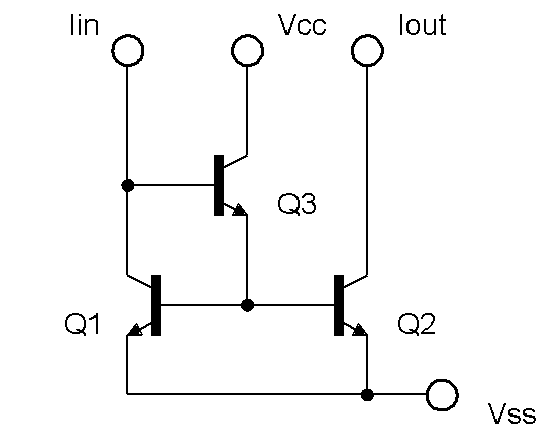
\includegraphics[scale=0.5]{pict/ZlepseneWilsonovoZrcadloNPN}
  \end{center}
  \caption[Wilson mirror]{Improved Wilson current mirror.}
\end{figure}

For inclusion of the vector-based graphics directly via \LaTeX, it is possible to use the \href{https://www.ctan.org/pkg/pgf}{\texttt{TikZ}} package.
Examples of use can be found at the \href{http://www.texample.net/tikz/examples/}{\TeX{}ample} site.
TikZ graphics creation is supported in QTikz and TikzEdt software.




\chapter{Examples of Listing Computer Codes}

\section{Package \texttt{listings}}

Listing computer codes can be handled efficiently via the \href{https://www.ctan.org/pkg/listings}{\texttt{listings}} package.
This package introduces a new environment \texttt{lstlisting} for typesetting computer codes, as for example:
%
\begin{lstlisting}[language={[LaTeX]TeX}]
\section{Package lstlistings}
Listing computer codes can be handled efficiently
via the \texttt{listings} package.
This package introduces a new environment
\texttt{lstlisting} for typesetting computer codes.
\end{lstlisting}
%
The package supports a number of programming languages.
The code to be typeset can be input directly from files on disk.
The package allows row numbering and extracting only selected parts of the code.
The following paragraph is an example of the use of \texttt{listings}:
\bigskip

\noindent
Abbreviations are typeset with the \texttt{acronym} environment:
\label{lst:abbrevs}
\lstinputlisting[language={[LaTeX]TeX}, nolol, numbers=left, firstnumber=6, firstline=6, lastline=6]{text/abbreviation.tex}
%
The width of the input parameter, \verb|HowMuchSpace|, determines the width of the first column.
An example of the definition of abbreviation \acs{symfs} is in Listing~\ref{lst:symfs}.

\shorthandoff{-}
\lstinputlisting%
	[language={[LaTeX]TeX}, frame=single, caption={[Example of code listing]Example of code listing.}, label=lst:symfs, numbers=left, linerange={bsymfvz-\%\%\%\ esymfvz}, includerangemarker=false]{text/abbreviation.tex}
\shorthandon{-}

\noindent
The list is finished with the end of the environment:
\lstinputlisting[language={[LaTeX]TeX}, nolol, numbers=left, firstnumber=26, linerange=26]{text/abbreviation.tex}

\vspace{\fill}

%\noindent
%{\bf Poznámka k~výpisům s~použitím volby jazyka \verb|czech| nebo \verb|slovak|:}\newline
%Pokud Váš zdrojový kód obsahuje znak spojovníku \verb|-|, pak překlad může skončit chybou.
%Ta je způsobená tím, že znak \verb|-| je v~českém nebo slovenském nastavení balíčku \verb|babel| tzv.\ aktivním znakem.
%Přepněte znak \verb|-| na neaktivní příkazem \verb|\shorthandoff{-}| těsně před výpisem a hned za ním jej vraťte na aktivní příkazem \verb|\shorthandon{-}|.
%Podobně jako to je ukázáno ve zdrojovém kódu šablony.


\clearpage

%\section{Listing Matlab code}
Listing \ref{lst:priklad.vypis.kodu.Matlab} contains an example of code for Matlab,
whereas in Listing \ref{lst:priklad.vypis.kodu.C} you find an example in the C~language.

\lstnewenvironment{matlab}[1][]{%
\lstset{language=Matlab,numbers=left,#1}%
}{%
}

\begin{matlab}%
	[frame=single, float=htbp, caption={[Example of the Schur--Cohn test of stability in Matlab]Example of the Schur--Cohn test of stability in Matlab.}, label=lst:priklad.vypis.kodu.Matlab, numberstyle=\scriptsize, numbersep=7pt]
%% Priklad testovani stability filtru

% koeficienty polynomu ve jmenovateli
a = [ 5, 11.2, 5.44, -0.384, -2.3552, -1.2288];
disp( 'Polynom:'); disp(poly2str( a, 'z'))

disp('Kontrola pomoci korenu polynomu:');
zx = roots( a);
if( all( abs( zx) < 1))
    disp('System je stabilni')
else
    disp('System je nestabilni nebo na mezi stability');
end

disp(' '); disp('Kontrola pomoci Schur-Cohn:');
ma = zeros( length(a)-1,length(a));
ma(1,:) = a/a(1);
for( k = 1:length(a)-2)
    aa = ma(k,1:end-k+1);
    bb = fliplr( aa);
    ma(k+1,1:end-k+1) = (aa-aa(end)*bb)/(1-aa(end)^2);
end

if( all( abs( diag( ma.'))))
    disp('System je stabilni')
else
    disp('System je nestabilni nebo na mezi stability');
end
\end{matlab}

\noindent
\begin{minipage}{\linewidth}


%\section{Listing C code}

\begin{lstlisting}%
	[frame=single, numbers=right, caption={[Example of implementation of first canonical form in~C]Example of implementation of first canonical form in~C.}, label=lst:priklad.vypis.kodu.C, basicstyle=\ttfamily\small, keywordstyle=\color{black}\bfseries\underbar]
// first canonical form
short fxdf2t( short coef[][5], short sample)
{
	static int v1[SECTIONS] = {0,0},v2[SECTIONS] = {0,0};
	int x, y, accu;
	short k;

	x = sample;
	for( k = 0; k < SECTIONS; k++){
		accu = v1[k] >> 1;
		y = _sadd( accu, _smpy( coef[k][0], x));
		y = _sshl(y, 1) >> 16;

		accu = v2[k] >> 1;
		accu = _sadd( accu, _smpy( coef[k][1], x));
		accu = _sadd( accu, _smpy( coef[k][2], y));
		v1[k] = _sshl( accu, 1);

		accu = _smpy( coef[k][3], x);
		accu = _sadd( accu, _smpy( coef[k][4], y));
		v2[k] = _sshl( accu, 1);

		x = y;
	}
	return( y);
}
\end{lstlisting}
\end{minipage}







\chapter{Content of the electronic attachment}
An electronic attachment is often a~part of the thesis.
The attachment is uploaded in the BUT information system together with the thesis PDF.
Please use an appropriate file format for the attachment.

It is suggested to comment on every folder, to specify which of the files contains main settings,
to specify which is the main or executable file, what was the setting of the compiler etc.
It is also valuable to specify in which version of the software the code has been tested (e.g.\ Matlab 2018b).
In the case that hardware has been created within the thesis, the electronic attachment must contain all documentation
(for example Eagle files with the printed circuit board layout).

If your attachment contains a~lot of files or folders,
\LaTeX{} package \href{https://www.ctan.org/pkg/dirtree}{\texttt{dirtree}} can become handy,
as in the following example.

\bigskip

{\small
%
\dirtree{%.
.1 /\DTcomment{root of the attached archive}.
.2 logo\DTcomment{logotypes}.
.3 BUT\_abbreviation\_color\_PANTONE\_EN.pdf.
.3 BUT\_color\_PANTONE\_EN.pdf.
.3 FEEC\_abbreviation\_color\_PANTONE\_EN.pdf.
.3 UTKO\_color\_PANTONE\_EN.pdf.
.2 pdf\DTcomment{PDFs (generate them in the information system)}.
.3 assignment-example.pdf.
.3 cover-example.pdf.
.3 titlepage-example.pdf.
.2 pict\DTcomment{other graphic files}.
.3 soucastky.png.
.3 spoje.png.
.3 ZlepseneWilsonovoZrcadloNPN.png.
.3 ZlepseneWilsonovoZrcadloPNP.png.
.2 text\DTcomment{\LaTeX{} source codes of the text}.
.3 abbreviation.tex.
.3 appendix.tex.
.3 bibliography.tex.
.3 conclusion.tex.
.3 introduction.tex.
.3 results.tex.
.3 solution.tex.
.2 template-thesis.tex\DTcomment{main file of the thesis}.
.2 template-presentation.tex\DTcomment{main file of the slides for presentation}.
.2 thesis.sty\DTcomment{package for typesetting final theses at BUT}.
}
}


\end{document}